\documentclass[tikz,border=2pt]{standalone}
\usepackage{amsmath,amssymb}
\usepackage{pgfplots}
\pgfplotsset{compat=1.18}
\usetikzlibrary{arrows.meta}
\begin{document}
% Jensen for a concave (logarithmic) utility: wealth W equals w_1 or w_2 with probability 1/2;
% E[u(W)] is the chord midpoint, which lies below u(E[W]) on the curve.
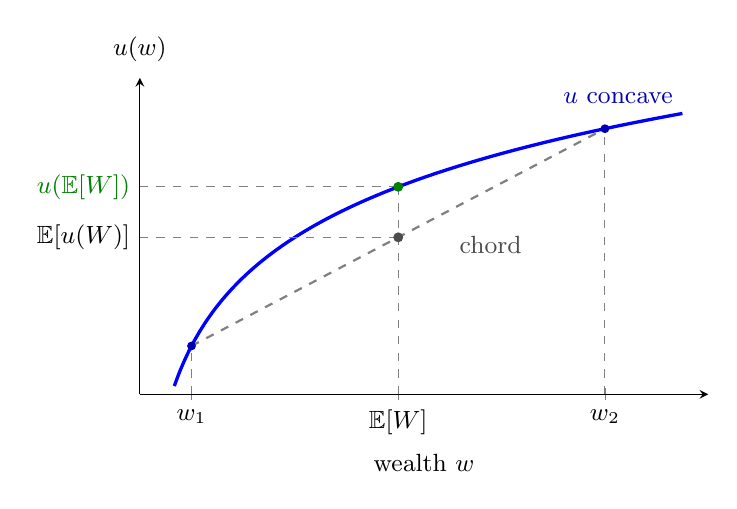
\begin{tikzpicture}[font=\small, >={Latex[length=2mm]}]
  \begin{axis}[
    axis lines=left, xmin=0, xmax=6.6, ymin=-1.0, ymax=2.2,
    xtick={0.6,3,5.4}, xticklabels={$w_1$,$\mathbb E[W]$,$w_2$}, ytick=\empty,
    xlabel={wealth $w$}, ylabel={$u(w)$},
    ylabel style={rotate=-90, anchor=south, at={(axis description cs:0,1.02)}},
    samples=120, smooth, width=8.8cm, height=5.6cm, clip=false]
    \addplot[blue, very thick, domain=0.4:6.3] {ln(x)};
    \node[blue!70!black, anchor=south east] at (axis cs:6.3,1.84) {$u$ concave};
    % chord between the two outcomes
    \draw[gray, thick, dashed] (axis cs:0.6,-0.5108) -- (axis cs:5.4,1.6864);
    \draw[gray, thin, dashed] (axis cs:0.6,-1.0) -- (axis cs:0.6,-0.5108);
    \draw[gray, thin, dashed] (axis cs:5.4,-1.0) -- (axis cs:5.4,1.6864);
    \draw[gray, thin, dashed] (axis cs:3,-1.0) -- (axis cs:3,1.0986);
    \fill[blue!70!black] (axis cs:0.6,-0.5108) circle (1.6pt);
    \fill[blue!70!black] (axis cs:5.4,1.6864) circle (1.6pt);
    % the two expected values at E[W]
    \draw[gray, thin, dashed] (axis cs:0,1.0986) -- (axis cs:3,1.0986);
    \draw[gray, thin, dashed] (axis cs:0,0.5878) -- (axis cs:3,0.5878);
    \fill[green!50!black] (axis cs:3,1.0986) circle (1.8pt);
    \fill[gray!60!black] (axis cs:3,0.5878) circle (1.8pt);
    \node[green!50!black, anchor=east] at (axis cs:0,1.0986) {$u(\mathbb E[W])$};
    \node[anchor=east] at (axis cs:0,0.5878) {$\mathbb E[u(W)]$};
    \node[gray!60!black, anchor=north west, font=\small] at (axis cs:3.6,0.70) {chord};
  \end{axis}
\end{tikzpicture}
\end{document}
